%%%%%%%%%%%%%%%%%%%%%%%%%%%%%%%%%%%%%%%%%
% Digital Processing Lab Template
% LaTeX Template
%
% This template has been downloaded from:
% http://www.LaTeXTemplates.com
%
% Original author:
% Linux and Unix Users Group at Virginia Tech Wiki 
% (https://vtluug.org/wiki/Example_LaTeX_chem_lab_report)
%
% License:
% CC BY-NC-SA 3.0 (http://creativecommons.org/licenses/by-nc-sa/3.0/)
%
%%%%%%%%%%%%%%%%%%%%%%%%%%%%%%%%%%%%%%%%%

%----------------------------------------------------------------------------------------
%	PACKAGES AND DOCUMENT CONFIGURATIONS
%----------------------------------------------------------------------------------------

\documentclass{article}

\usepackage[version=3]{mhchem} % Package for chemical equation typesetting
\usepackage{siunitx} % Provides the \SI{}{} and \si{} command for typesetting SI units
\usepackage{polski}
\usepackage[utf8]{inputenc}
\DeclareUnicodeCharacter{00A0}{~}
\usepackage[table]{xcolor}% http://ctan.org/pkg/xcolor
\usepackage{graphicx} % Required for the inclusion of images
\usepackage{natbib} % Required to change bibliography style to APA
\usepackage{amsmath} % Required for some math elements 

\setlength\parindent{0pt} % Removes all indentation from paragraphs
\addtolength{\oddsidemargin}{-.875in} % decreasing margin size
\addtolength{\evensidemargin}{-.875in}
\addtolength{\textwidth}{1.75in}
\addtolength{\topmargin}{-.875in}
\addtolength{\textheight}{1.75in}

\renewcommand{\labelenumi}{\alph{enumi}.} % Make numbering in the enumerate environment by letter rather than number (e.g. section 6)
\renewcommand{\figurename}{Rysunek}

%--------------- WSTAWIANIE KODU ------------------------%
\usepackage{listings}
\usepackage{color}

\definecolor{mygreen}{rgb}{0,0.6,0}
\definecolor{mygray}{rgb}{0.5,0.5,0.5}
\definecolor{mymauve}{rgb}{0.58,0,0.82}

\lstset{ %
  backgroundcolor=\color{white},   % choose the background color; you must add \usepackage{color} or \usepackage{xcolor}
  basicstyle=\footnotesize,        % the size of the fonts that are used for the code
  breakatwhitespace=false,         % sets if automatic breaks should only happen at whitespace
  breaklines=true,                 % sets automatic line breaking
  captionpos=b,                    % sets the caption-position to bottom
  commentstyle=\color{mygreen},    % comment style
  deletekeywords={...},            % if you want to delete keywords from the given language
  escapeinside={\%*}{*)},          % if you want to add LaTeX within your code
  extendedchars=true,              % lets you use non-ASCII characters; for 8-bits encodings only, does not work with UTF-8
  frame=single,                    % adds a frame around the code
  keepspaces=true,                 % keeps spaces in text, useful for keeping indentation of code (possibly needs columns=flexible)
  keywordstyle=\color{blue},       % keyword style
  language={[x86masm]Assembler},                 % the language of the code
  otherkeywords={*,...},            % if you want to add more keywords to the set
  numbers=left,                    % where to put the line-numbers; possible values are (none, left, right)
  numbersep=5pt,                   % how far the line-numbers are from the code
  numberstyle=\tiny\color{mygray}, % the style that is used for the line-numbers
  rulecolor=\color{black},         % if not set, the frame-color may be changed on line-breaks within not-black text (e.g. comments (green here))
  showspaces=false,                % show spaces everywhere adding particular underscores; it overrides 'showstringspaces'
  showstringspaces=false,          % underline spaces within strings only
  showtabs=false,                  % show tabs within strings adding particular underscores
  stepnumber=2,                    % the step between two line-numbers. If it's 1, each line will be numbered
  stringstyle=\color{mymauve},     % string literal style
  tabsize=2,                       % sets default tabsize to 2 spaces
  title=\lstname                   % show the filename of files included with \lstinputlisting; also try caption instead of title
}



%-------------------------------------------------------------%

%\usepackage{times} % Uncomment to use the Times New Roman font

%----------------------------------------------------------------------------------------
%	DOCUMENT INFORMATION
%----------------------------------------------------------------------------------------

\title{Laboratorium techniki mikroprocesorowej \\ Ćwiczenie 4 \\ Przetworniki A/C i C/A} % Title

\author{Rafał \textsc{Grabiański} \\ Zbigniew \textsc{Królikowski}} % Author name

\date{\today} % Date for the report

\begin{document}

\maketitle % Insert the title, author and date

\begin{center}
\begin{tabular}{l r}
Data wykonania: & 24 kwietnia 2015 \\ % Date the experiment was performed
\end{tabular}
\end{center}

% If you wish to include an abstract, uncomment the lines below
% \begin{abstract}
% Abstract text
% \end{abstract}

%----------------------------------------------------------------------------------------
%	SECTION 1 - CEL ĆWICZENIA
%----------------------------------------------------------------------------------------

\section{Cel ćwiczenia}
Celem ćwiczenia było zapoznanie się z budową i zasadą działania wybranych rodzajów przetworników
analogowo-cyfrowych (A/C) oraz cyfrowo-analogowych (C/A).
 
%----------------------------------------------------------------------------------------
%	SECTION 2 - Wykonanie ćwiczenia
%----------------------------------------------------------------------------------------

\section{Wykonanie ćwiczenia}

\subsection{Obserwacja działania komparatora analogowego}
\subsubsection{Komparator analogowy bez histerezy}
Połączyliśmy wyjścia zadajnika z wejściami komparatora, a wyjście komparatora do wejścia pomiarowego
zadajnika. Na wejścia IN+ podaliśmy napięcie 1.5V. Pętla histerezy była wyłączona. Następnie powoli zwiększaliśmy
wartość napięcia IN- z 0V do 2.5V obserwując, kiedy zmieni się napięcia na wyjściu i równocześnie stan diody na płytce
komparatora. Następnie robiliśmy odwrotnie, zmniejszając napięcie do 0V.

\begin{figure}[h!]
	\centering
	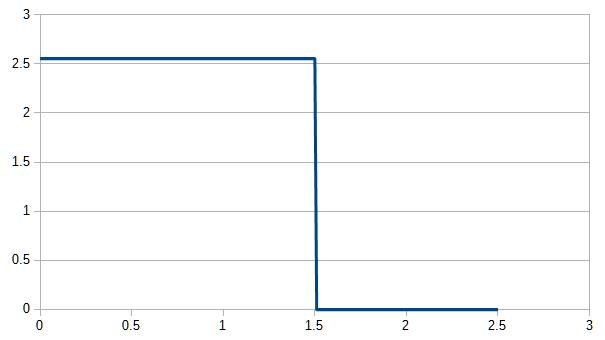
\includegraphics[scale=0.5]{ch01}
\end{figure}
\clearpage
\subsubsection{Komparator analogowy z histerezą}
Następnie wykonaliśmy te samo ćwiczenie z tym, że tym razem z włączoną pętlą histerezy. 
\begin{figure}[h!]
	\centering
	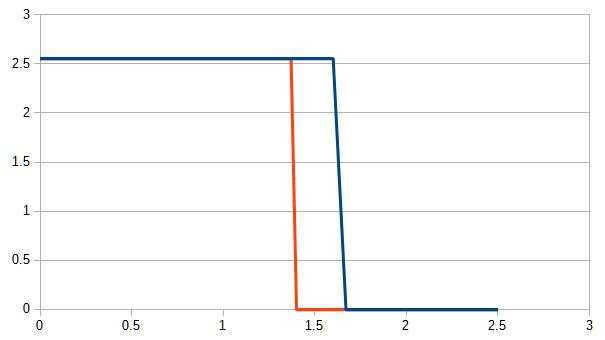
\includegraphics[scale=0.4]{ch02}
\end{figure}

\subsection{Obserwacja statycznego działania przetwornika A/C}
Podłączyliśmy wejścia przetwornika A/C z wyjściami zadajnika. Ustawiliśmy napięcie referencyjne na poziomie 1.6V.
Napięcie podawane na wejście $V_{in}$ zmienialiśmy od 0V do 1.6V.
\begin{figure}[h!]
	\centering
	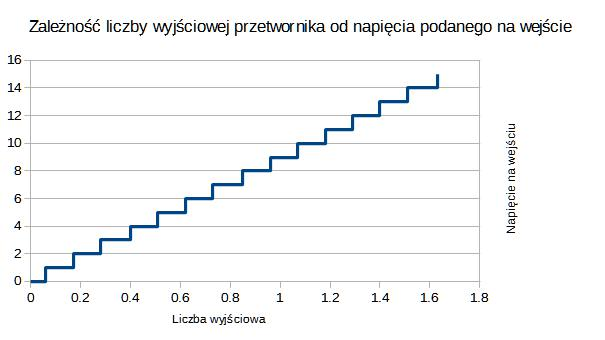
\includegraphics[scale=0.4]{ch03}
\end{figure}


\subsection{Obserwacja statycznego działania przetwornika C/A}
Połączyliśmy moduł przełączników z wejściem cyfrowym przetwornika C/A. Filtr dolnoprzepustowy był podczas tej obserwacji
wyłączony.
\begin{figure}[h!]
	\centering
	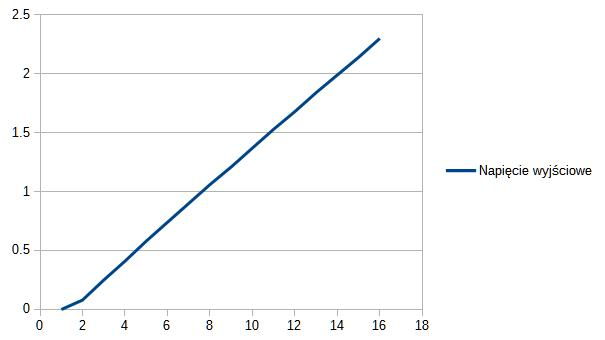
\includegraphics[scale=0.35]{ch04}
\end{figure}

\clearpage
\subsection{Obserwacja dynamicznego działania przetwornika C/A}
\label{subsec:dynamiczne_C/A}
Widać wyraźne schodki przy wyłączonym filtrze dolnoprzepustowym, następnie przy włączonym przebieg staje się
wygładzony. Filtr dolnoprzepustowy umożliwia ograniczenie zjawiska aliasingu. Np. w cyfrowych aparatach filtr taki lekko rozmywa obraz padający na przetwornik.

\begin{figure}[h!]
	\centering
	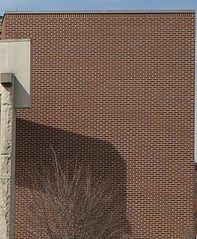
\includegraphics[scale=0.65]{img1}
	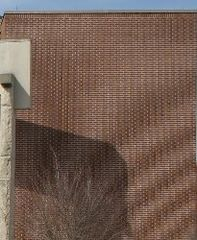
\includegraphics[scale=0.65]{img2}
	\caption{Na drugim zdjęciu widoczne zjawisko aliasingu}
\end{figure}

\begin{figure}[h!]
	\centering
	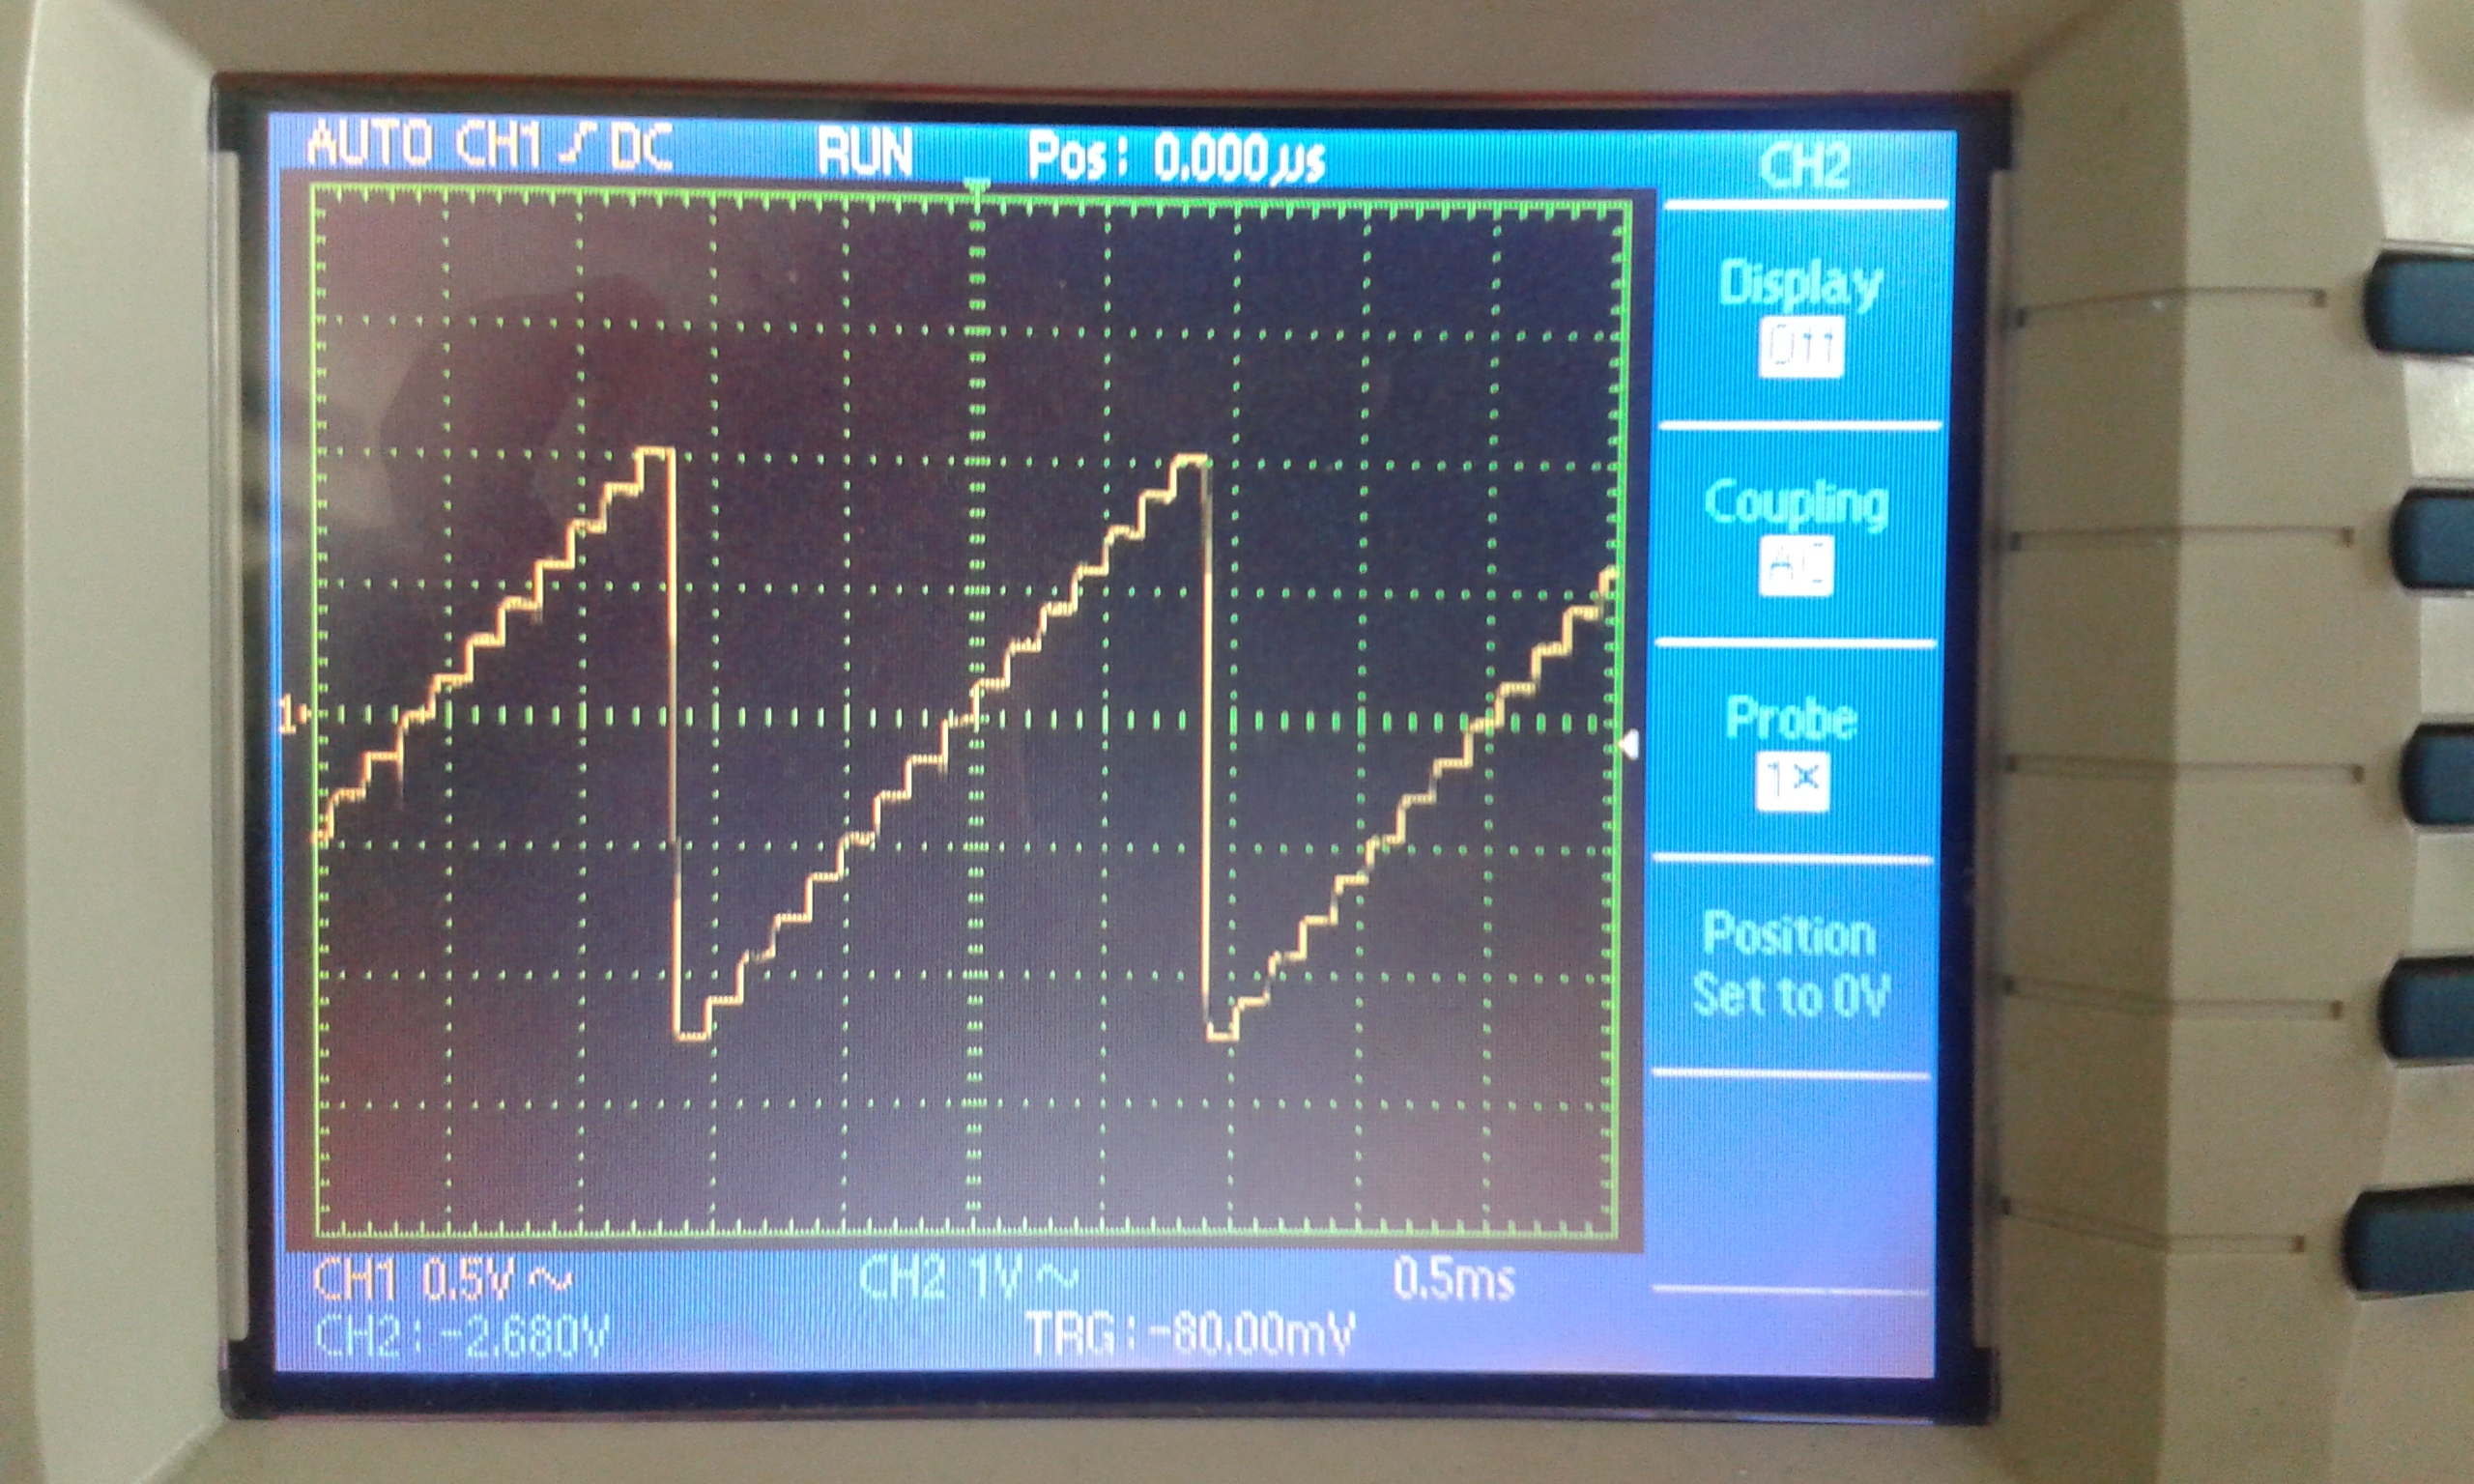
\includegraphics[scale=0.1]{img3}
	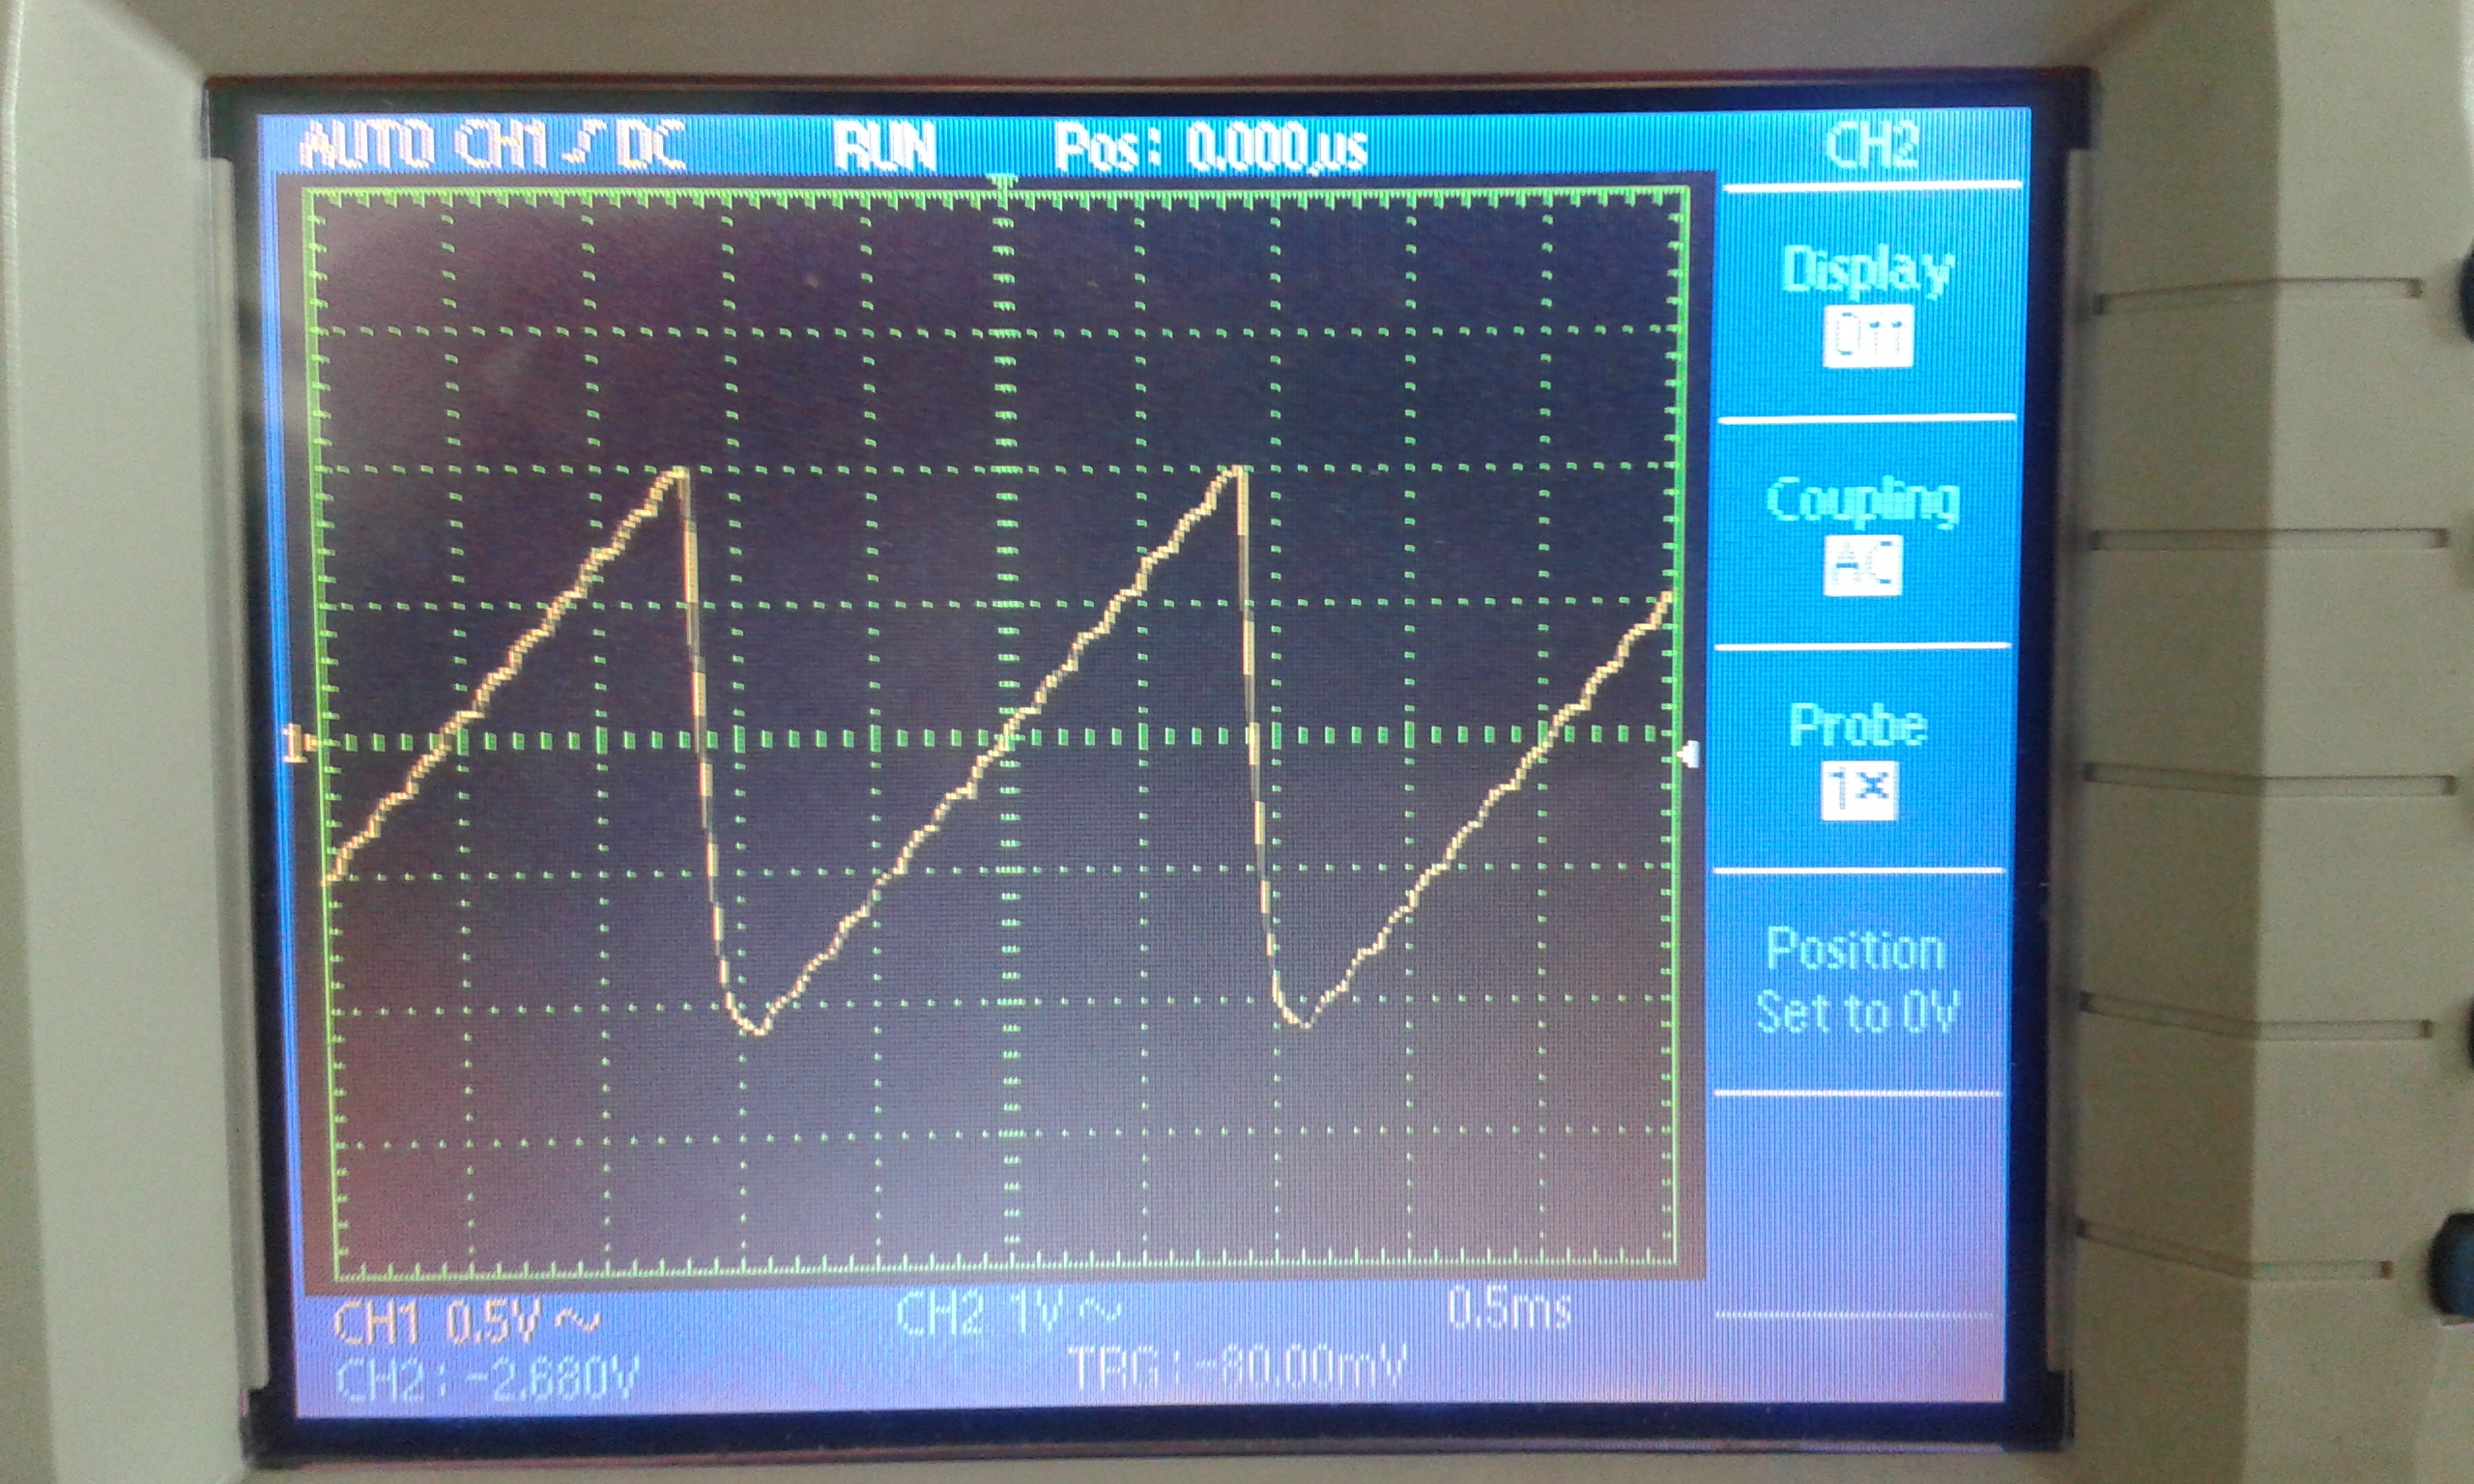
\includegraphics[scale=0.1]{img4}
	\caption{Przebieg zarejestrowany na oscyloskopie. Na górze z wył. filtrem, na dole włączony.}
\end{figure}

\subsection{Obserwacja statyczna toru przetwarzania A/C-C/A}
Połączyliśmy ze sobą przetwornik A/C i C/A, na wejście A/C podaliśmy napięcie 2.5V. Na zadajniku mierzyliśmy
napięcie wyjściowe z modułu C/A. Maksymalna zaobserwowana różnica to 0.28V i zaszła ona dla napięcia wejściowego 2.25V, przy czym napięcie za przetwornikiem C/A wyniosło wtedy 1.97V.

\subsection{Obserwacja dynamiczna toru przetwarzania A/C-C/A}
Tym razem do podłączonych modułów A/C-C/A podaliśmy na wejście sygnał sinusoidalny o częstotliwości 500Hz, amplitudzie 2V i offsecie 1.1V. Sygnał ten generowany był przez płytę testową NI ELVIS II sterowaną za pomocą aplikacji na komputerze.

\begin{figure}[h!]
	\centering
	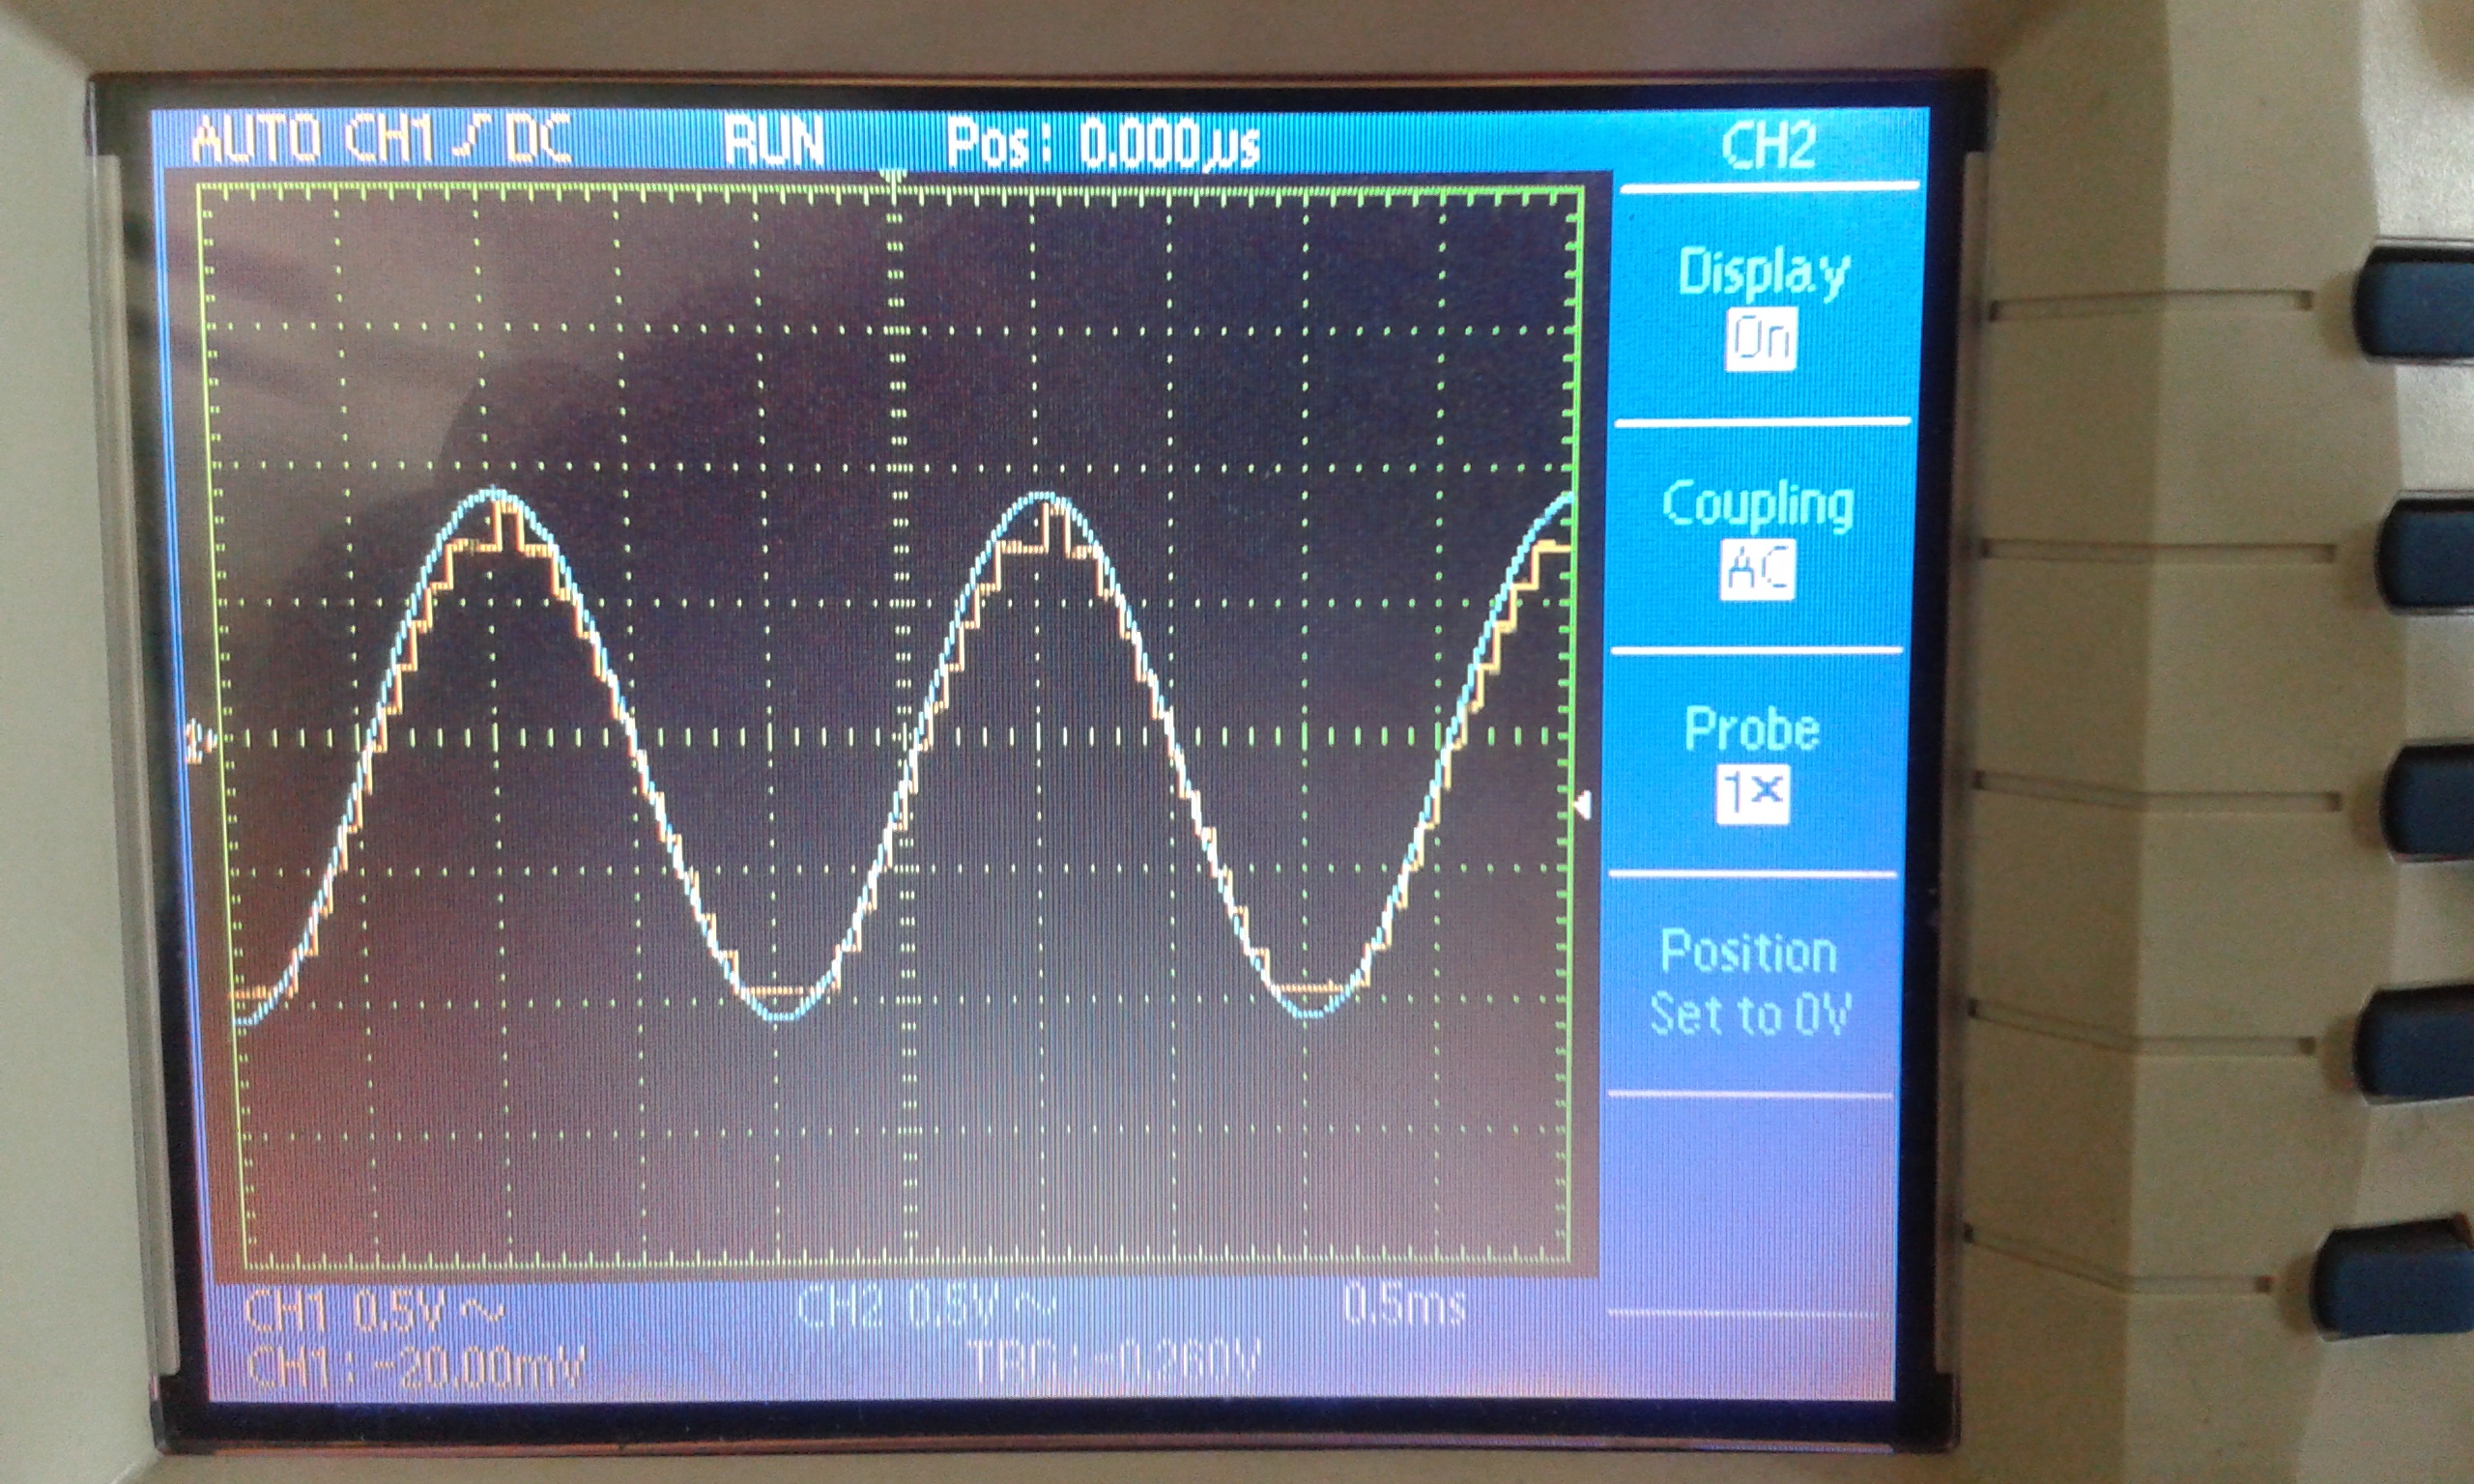
\includegraphics[scale=0.1]{img5}
	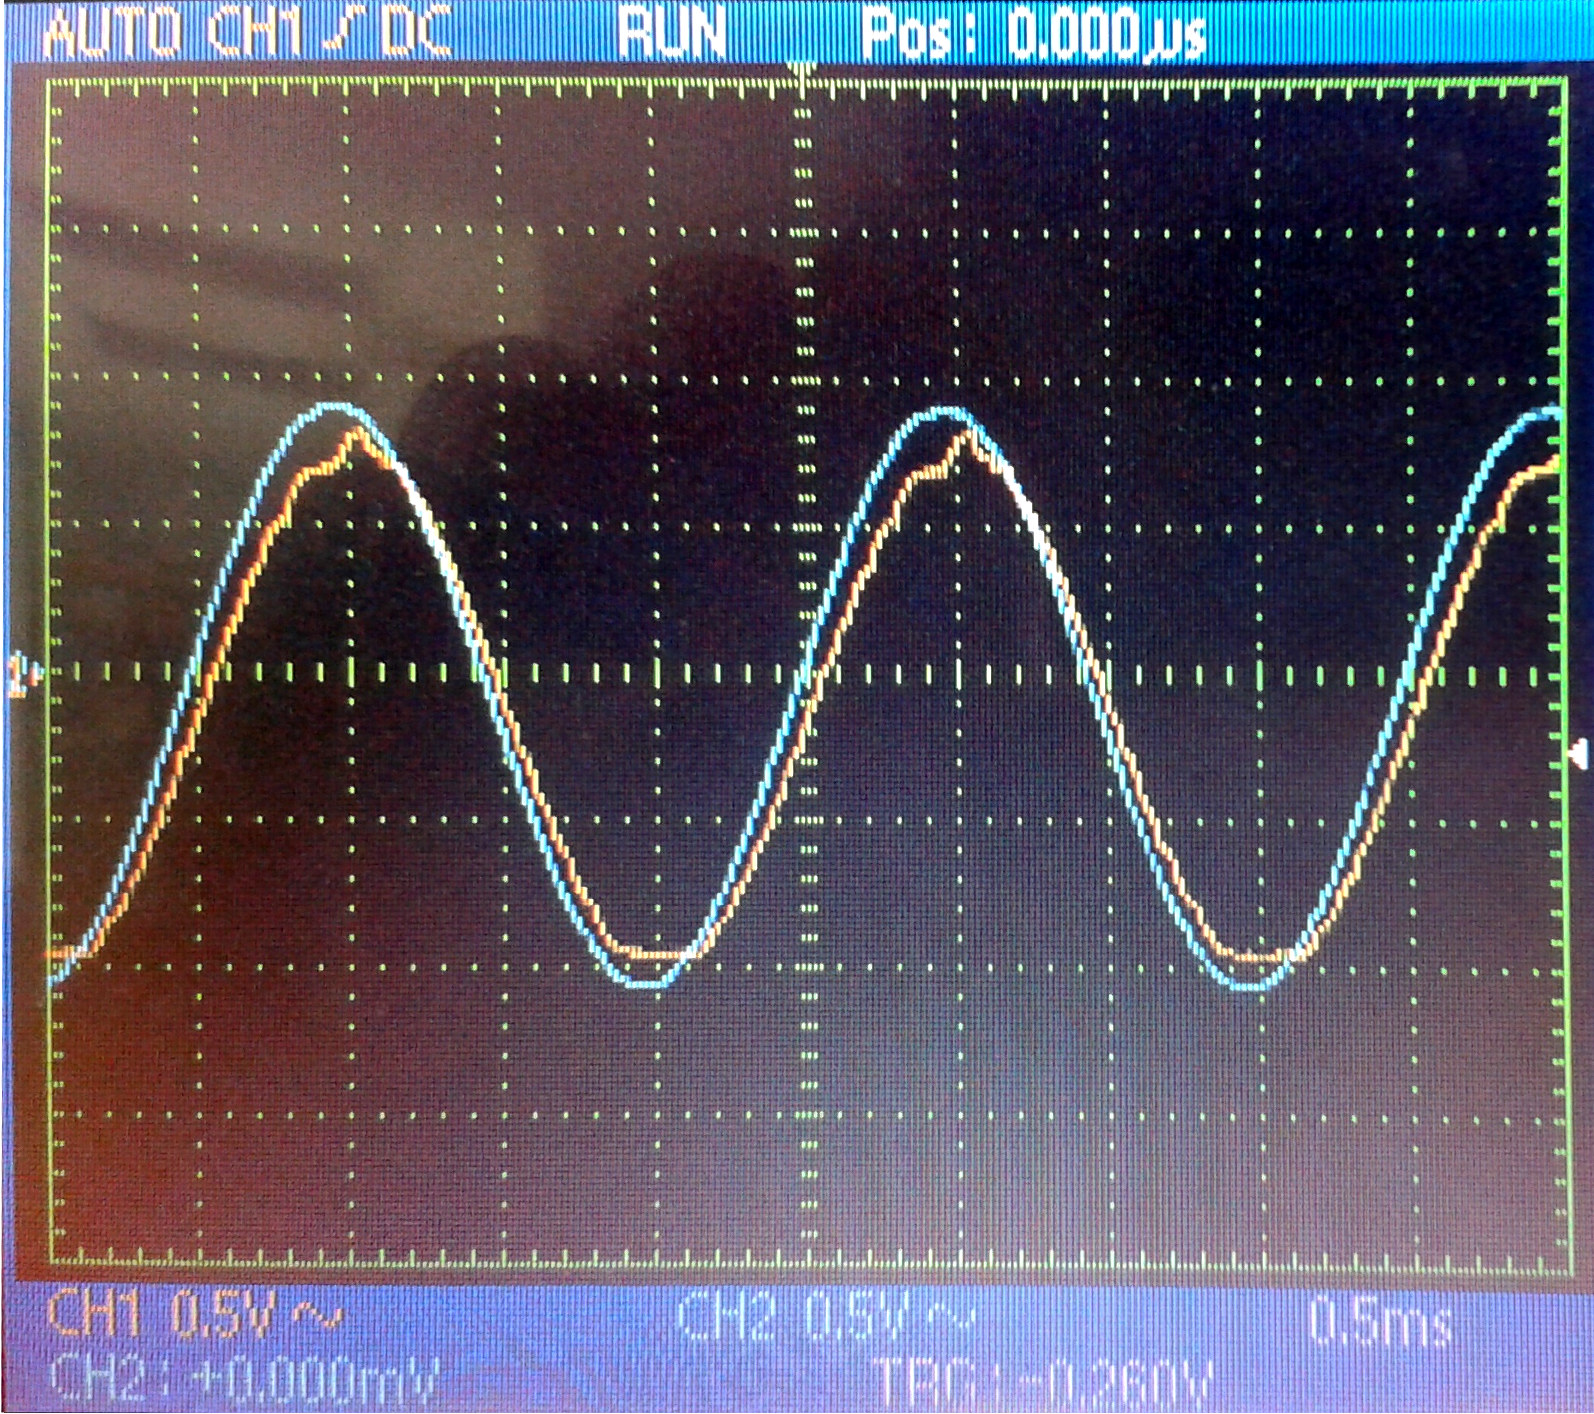
\includegraphics[scale=0.1]{img6}
	\caption{Przebiegi zarejestrowane na oscyloskopie. Na górze z wyłączonym filtrem dolnoprzepustowy, na dole z włączonym. Na niebiesko przebieg wejściowy, na żółto wyjście z C/A.}
\end{figure}

Wnioski są w zasadzie podobne do tych w punkcie ~\ref{subsec:dynamiczne_C/A}. Filtr dolnoprzpustowy odcina część częstotliwości poniżej granicznej, w wyniku czego wykres staje się bardziej gładki.

%----------------------------------------------------------------------------------------
%	BIBLIOGRAPHY
%----------------------------------------------------------------------------------------

\bibliographystyle{apalike}

\bibliography{sample}

%----------------------------------------------------------------------------------------


\end{document}